\documentclass[12pt]{article}

\usepackage[top=5em, bottom=5em, left=5em, right=5em]{geometry}
\usepackage{tikz}
\usetikzlibrary{positioning}

\setlength\parindent{0em}
\setlength\parskip{1em}

\title {Assignment 3}

\author {Hendrik Werner s4549775}

\begin{document}
\maketitle

This was done in collaboration with Constantin Blach (s4329872).

\section{} %1
Initial state:

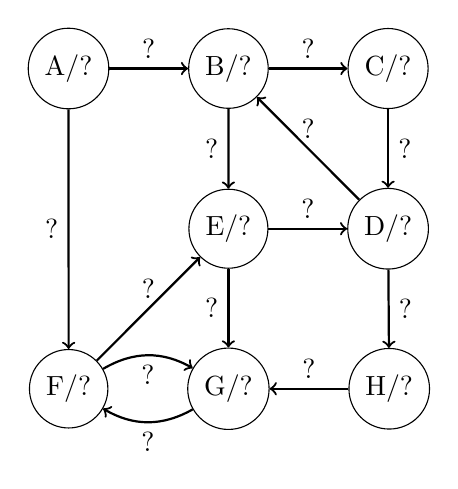
\begin{tikzpicture}[c/.style={circle, draw}]
	\node [c] (A) {A/?};
	\node [c, right=of A] (B) {B/?};
	\node [c, right=of B] (C) {C/?};
	\node [c, below=of C] (D) {D/?};
	\node [c, left =of D] (E) {E/?};
	\node [c, below=of E] (G) {G/?};
	\node [c, left =of G] (F) {F/?};
	\node [c, right=of G] (H) {H/?};

	\path[->, thick] (A) edge node [above] {?} (B);
	\path[->, thick] (A) edge node [left ] {?} (F);
	\path[->, thick] (B) edge node [above] {?} (C);
	\path[->, thick] (B) edge node [left ] {?} (E);
	\path[->, thick] (C) edge node [right] {?} (D);
	\path[->, thick] (D) edge node [above] {?} (B);
	\path[->, thick] (D) edge node [right] {?} (H);
	\path[->, thick] (E) edge node [above] {?} (D);
	\path[->, thick] (E) edge node [left ] {?} (G);
	\path[->, thick] (F) edge node [above] {?} (E);
	\path[->, thick] (F) edge [bend left] node [below] {?} (G);
	\path[->, thick] (G) edge [bend left] node [below] {?} (F);
	\path[->, thick] (H) edge node [above] {?} (G);
\end{tikzpicture}

\begin{enumerate}
	\item
	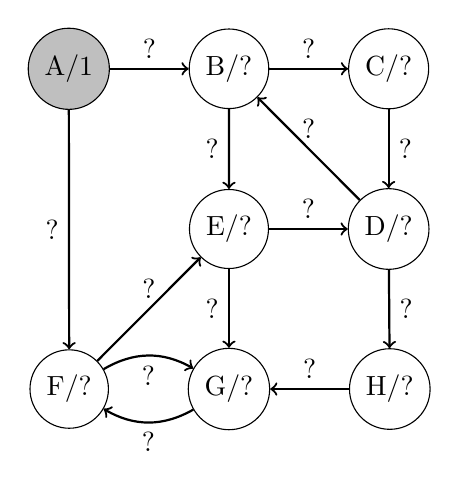
\begin{tikzpicture}[c/.style={circle, draw}, visited/.style={fill=lightgray}]
		\node [c, visited] (A) {A/1};
		\node [c, right=of A] (B) {B/?};
		\node [c, right=of B] (C) {C/?};
		\node [c, below=of C] (D) {D/?};
		\node [c, left =of D] (E) {E/?};
		\node [c, below=of E] (G) {G/?};
		\node [c, left =of G] (F) {F/?};
		\node [c, right=of G] (H) {H/?};

		\path[->, thick] (A) edge node [above] {?} (B);
		\path[->, thick] (A) edge node [left ] {?} (F);
		\path[->, thick] (B) edge node [above] {?} (C);
		\path[->, thick] (B) edge node [left ] {?} (E);
		\path[->, thick] (C) edge node [right] {?} (D);
		\path[->, thick] (D) edge node [above] {?} (B);
		\path[->, thick] (D) edge node [right] {?} (H);
		\path[->, thick] (E) edge node [above] {?} (D);
		\path[->, thick] (E) edge node [left ] {?} (G);
		\path[->, thick] (F) edge node [above] {?} (E);
		\path[->, thick] (F) edge [bend left] node [below] {?} (G);
		\path[->, thick] (G) edge [bend left] node [below] {?} (F);
		\path[->, thick] (H) edge node [above] {?} (G);
	\end{tikzpicture}

	\item
	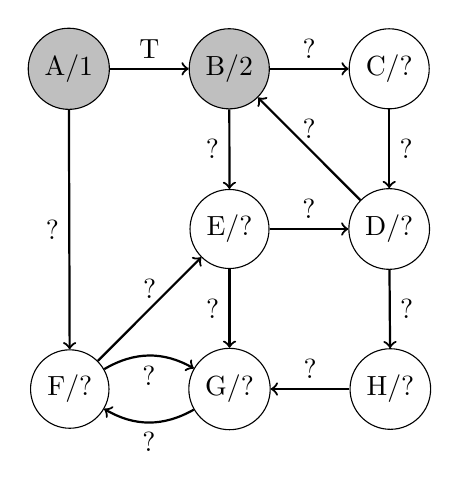
\begin{tikzpicture}[c/.style={circle, draw}, visited/.style={fill=lightgray}]
		\node [c, visited] (A) {A/1};
		\node [c, visited, right=of A] (B) {B/2};
		\node [c, right=of B] (C) {C/?};
		\node [c, below=of C] (D) {D/?};
		\node [c, left =of D] (E) {E/?};
		\node [c, below=of E] (G) {G/?};
		\node [c, left =of G] (F) {F/?};
		\node [c, right=of G] (H) {H/?};

		\path[->, thick] (A) edge node [above] {T} (B);
		\path[->, thick] (A) edge node [left ] {?} (F);
		\path[->, thick] (B) edge node [above] {?} (C);
		\path[->, thick] (B) edge node [left ] {?} (E);
		\path[->, thick] (C) edge node [right] {?} (D);
		\path[->, thick] (D) edge node [above] {?} (B);
		\path[->, thick] (D) edge node [right] {?} (H);
		\path[->, thick] (E) edge node [above] {?} (D);
		\path[->, thick] (E) edge node [left ] {?} (G);
		\path[->, thick] (F) edge node [above] {?} (E);
		\path[->, thick] (F) edge [bend left] node [below] {?} (G);
		\path[->, thick] (G) edge [bend left] node [below] {?} (F);
		\path[->, thick] (H) edge node [above] {?} (G);
	\end{tikzpicture}
\end{enumerate}

\section{} %2
\section{} %3
\section{} %4
\section{} %5
\section{} %6

\end{document}
